\chapter{Installation}
\label{chapter:Installation}
\index{Installation}

This section describes the process for installing ITK on your system. Keep in
mind that ITK is a toolkit, and as such, once it is installed in your computer
there will be no application to run. Rather, you will use ITK to build your
own applications. What ITK does provide---besides the toolkit proper---is a
large set of test files and examples that will introduce you to ITK concepts
and will show you how to use ITK in your own projects.

Some of the examples distributed with ITK require third party libraries that
you may have to download. For an initial installation of ITK you may want to
ignore these extra libraries and just build the toolkit itself. In the past,
a large fraction of the traffic on the insight-users mailing list has
originated from
difficulties in getting third party libraries compiled and installed rather
than with actual problems building ITK.

ITK has been developed and tested across different combinations of
operating systems, compilers, and hardware platforms including
MS-Windows, Linux on Intel-compatible hardware, Solaris, IRIX, Mac
OSX, and Cygwin.  It is known to work with the following compilers:

\begin{itemize}
\item Visual Studio 6, .NET 2002, .NET 2003
\item GCC 2.95.x, 2.96, 3.x
\item SGI MIPSpro 7.3x
\item Borland 5.5
\end{itemize}

Given the advanced usage of C++ features in the toolkit, some
compilers may have difficulties processing the code. If you are
currently using an outdated compiler this may be an excellent excuse
for upgrading this old piece of software!

\section{Configuring ITK}
\label{sec:ConfiguringITK}

\index{Configuration}
 
The challenge of supporting ITK across platforms has been solved through the
use of CMake, a cross-platform, open-source build system. CMake is used to
control the software compilation process using simple platform and compiler
independent configuration files.  CMake generates native makefiles and
workspaces that can be used in the compiler environment of your choice. CMake
is quite sophisticated---it supports complex environments requiring system
configuration, compiler feature testing, and code generation.

CMake generates Makefiles under UNIX and Cygwin systems and generates Visual
Studio workspaces under Windows (and appropriate build files for other
compilers like Borland). The information used by CMake is provided by
\code{CMakeLists.txt} files that are present in every directory of the ITK
source tree. These files contain information that the user
provides to CMake at configuration time. Typical information includes paths
to utilities in the system and the selection of software options specified by
the user.

\subsection{Preparing CMake}
\label{sec:CMakeforITK}
 
\index{CMake}
\index{CMake!downloading}

CMake can be downloaded at no cost from 
\begin{center} 
  \url{http://www.cmake.org}
\end{center}

ITK requires at least CMake version 2.0. You can download binary
versions for most of the popular platforms including Windows, Solaris,
IRIX, HP, Mac and Linux. Alternatively you can download the source
code and build CMake on your system. Follow the instructions in the
CMake Web page for downloading and installing the software.

Running CMake initially requires that you provide two pieces of
information: where the source code directory is located
(ITK\_SOURCE\_DIR), and where the object code is to be produced
(ITK\_BINARY\_DIR). These are referred to as the \emph{source
directory} and the \emph{binary directory}. We recommend setting the
binary directory to be different than the source directory (an
\emph{out-of-source} build), but ITK will still build if they are set
to the same directory (an \emph{in-source} build).  On Unix, the
binary directory is created by the user and CMake is invoked with the
path to the source directory. For example:

\small
\begin{verbatim}
mkdir Insight-binary
cd Insight-binary
ccmake ../Insight
\end{verbatim}
\normalsize

On Windows, the CMake GUI is used to specify the source and build
directories (Figure \ref{fig:CMakeGUI}).

CMake runs in an interactive mode in that you iteratively select options and
configure according to these options. The iteration proceeds until no more
options remain to be selected. At this point, a generation step produces the appropriate
build files for your configuration.

This interactive configuration process can be better understood if you
imagine that you are walking through a decision tree.  Every option that you
select introduces the possibility that new, dependent options may become
relevant. These new options are presented by CMake at the top of the options
list in its interface.  Only when no new options appear after a configuration
iteration can you be sure that the necessary decisions have all been made. At
this point build files are generated for the current configuration.

\subsection{Configuring ITK}
\label{sec:ConfiguringITKwithVTK}
  
\index{Configuration!with VTK}

\begin{figure}[ht]
\centering 
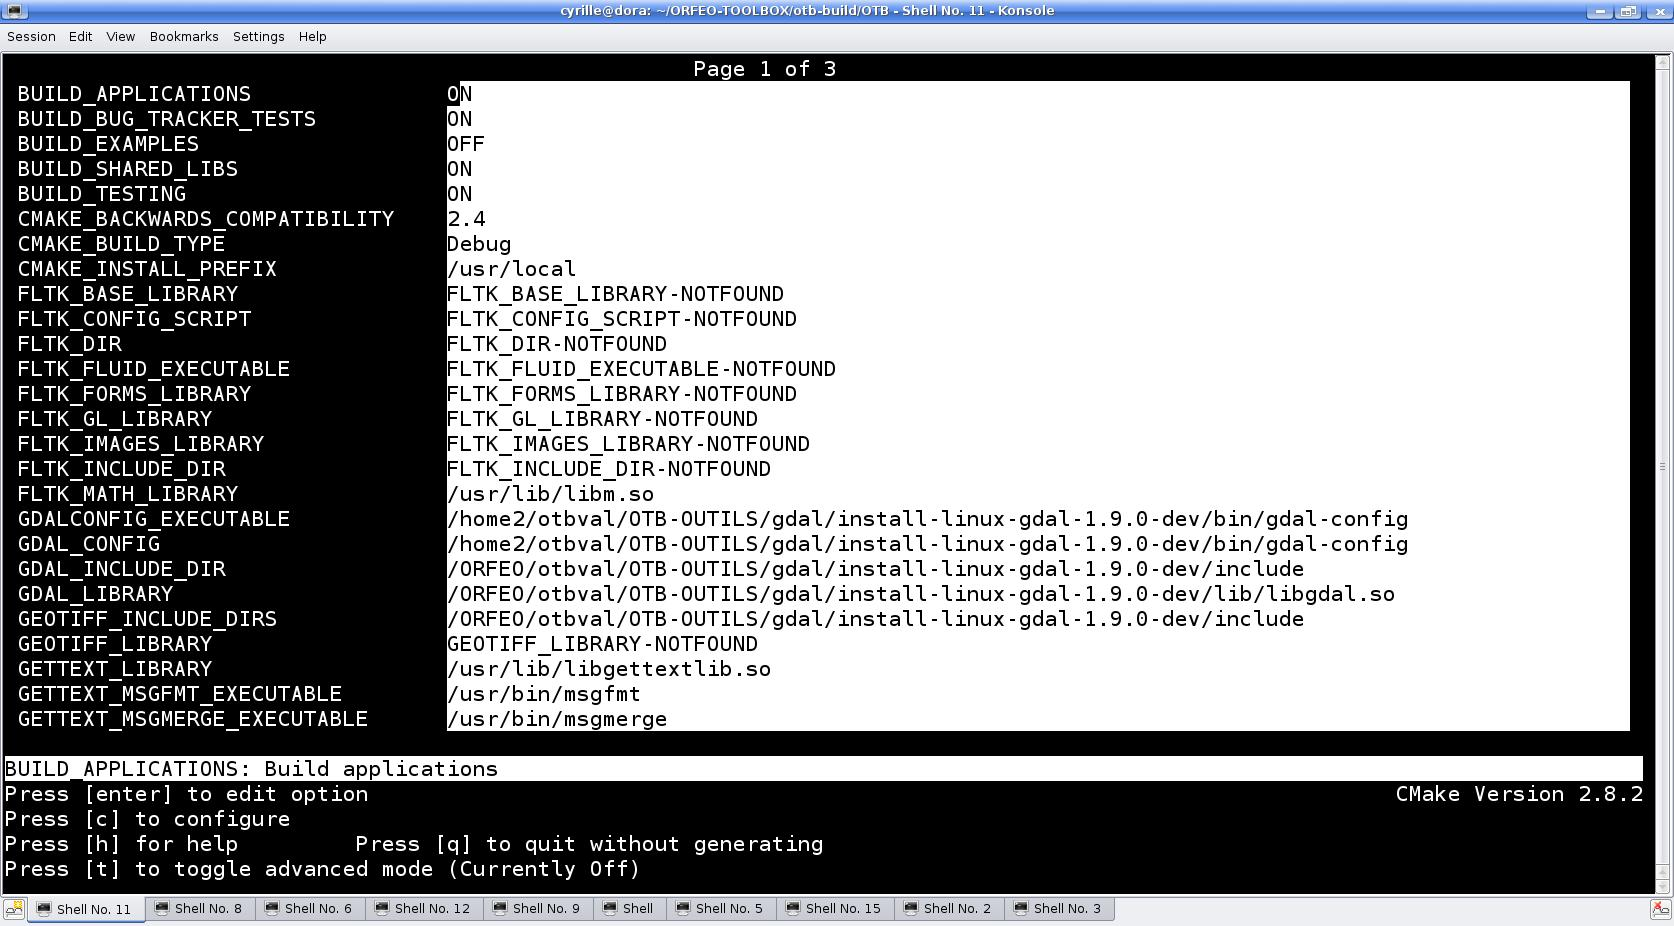
\includegraphics[width=0.8\textwidth]{ccmakeScreenShot.eps}
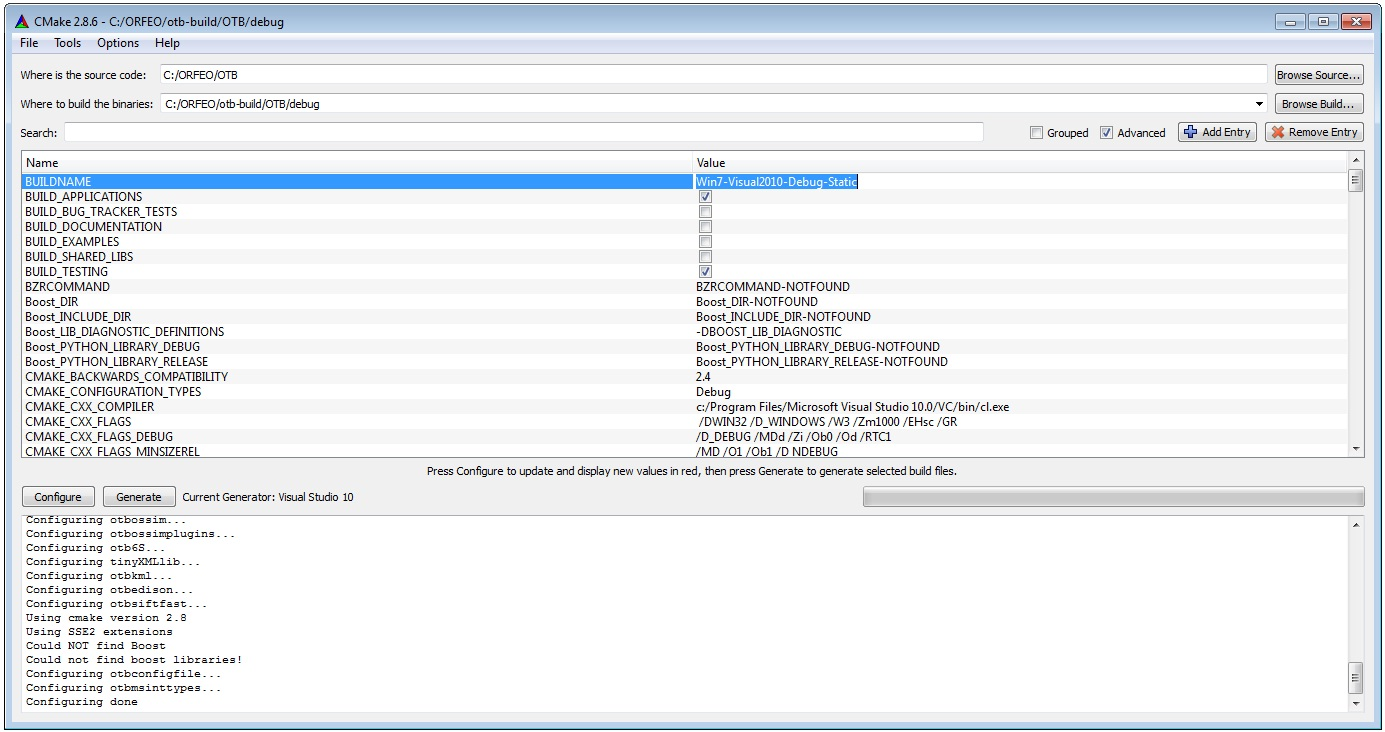
\includegraphics[width=0.8\textwidth]{CMakeSetupScreenShot.eps}
\itkcaption[Cmake user interface]{CMake interface. Top) \texttt{ccmake}, the UNIX
version based on \texttt{curses}. Bottom) \texttt{CMakeSetup}, the MS-Windows
version based on MFC.}
\label{fig:CMakeGUI}
\end{figure}

Figure \ref{fig:CMakeGUI} shows the CMake interface for UNIX and MS-Windows.
In order to speed up the build process you may want to disable the compilation
of the testing and examples. This is done with the variables
\code{BUILD\_TESTING=OFF} and \code{BUILD\_EXAMPLES=OFF}.  The examples
distributed with the toolkit are a helpful resource for learning how to use ITK
components but are not essential for the use of the toolkit itself. The testing
section includes a large number of small programs that exercise the
capabilities of ITK classes. Due to the large number of tests, enabling the
testing option will considerably increase the build time.  It is not
desirable to enable this option for a first build of the toolkit.

An additional resource is available in the \code{InsightApplications} module,
which contains multiple applications incorporating GUIs and different levels
of visualization.  However, due to the large number of applications and the
fact that some of them rely on third party libraries, building this module
should be postponed until you are familiar with the basic structure of the
toolkit and the building process. 

Begin running CMake by using
ccmake on Unix, and CMakeSetup on
Windows. Remember to run ccmake from the binary directory on Unix. On
Windows, specify the source and binary directories in the GUI, then begin to
set the build variables in the GUI as necessary.  Most variables should have
default values that are sensible. Each time you change a set of variables in
CMake, it is necessary to proceed to another configuration step. In the
Windows version this is done by clicking on the ``Configure'' button. In the
UNIX version this is done in an interface using the 
curses library, where you can configure by hitting the ``c'' key.

When no new options appear in CMake, you can proceed to generate Makefiles or
Visual Studio projects (or appropriate build file(s) depending on your
compiler). This is done in Windows by clicking on the ``Ok'' button.  In the
UNIX version this is done by hitting the ``g'' key. After the generation
process CMake will quit silently. To initiate the build process on UNIX,
simply type \code{make} in the binary directory. Under Windows, load the
workspace named \code{ITK.dsw} (if using MSDEV) or \code{ITK.sln} (if using
the .NET compiler) from the binary directory you specified in the CMake GUI.

The build process will typically take anywhere from 15 to 30 minutes depending
on the performance of your system. If you decide to enable testing as part of
the normal build process, about 600 small test programs will be compiled. This
will verify that the basic components of ITK have been correctly built on your
system.


\section{Getting Started With ITK }
\label{sec:GettingStartedWithITK}
 
The simplest way to create a new project with ITK is to create a new directory
somewhere in your disk and create two files in it. The first one is a
\code{CMakeLists.txt} file that will be used by CMake to generate a Makefile
(if you are using UNIX) or a Visual Studio workspace (if you are using
MS-Windows).  The second file is an actual C++ program that will exercise
some of the large number of classes available in ITK. The details of these files
are described in the following section.

Once both files are in your directory you can run CMake in order to configure
your project. Under UNIX, you can cd to your newly created directory
and type ``\code{ccmake .}''. Note the ``.'' in the command line for indicating
that the \code{CMakeLists.txt} file is in the current directory. The
curses interface will require you to provide the directory where ITK
was built. This is the same path that you indicated for the
\code{ITK\_BINARY\_DIR} variable at the time of configuring ITK. Under
Windows you can run CMakeSetup and provide your newly created
directory as being both the source directory and the binary directory for
your new project (i.e., an in-source build). Then CMake will require you to
provide the path to the binary directory where ITK was built. The ITK binary
directory will contain a file named \code{ITKConfig.cmake} generated during the
configuration process at the time ITK was built.  From this file, CMake will
recover all the information required to configure your new ITK project.

\subsection{Hello World !}
\label{sec:HelloWorldITK}

\index{Hello World}

\index{Installation}

Ce chapitre d\'{e}crit les proc\'{e}dures pour installer l'OTB sur votre syst\`{e}me.
Vous devez avant tout compiler l'OTB pour pouvoir l'utiliser et cr\'{e}er vos propres applications.


L'OTB s'appuie sur un ensemble de biblioth\`{e}ques externes de type libre (licence GNU/GPL, etc...) qu'il est n\'{e}cessaire de disposer sur votre syst\`{e}me.
Ces biblioth\`{e}ques sont les suivantes :
\begin{itemize}
\item ITK\footnote{http://www.itk.org} (\emph{Insight Toolkit}) utilis\'{e}e comme base de d\'{e}veloppement de l'OTB, pour tous les traitements de filtrage, recalage, segmentation, etc...
\item VTK\footnote{http://www.vtk.org} (\emph{Visualization ToolKit}) utilis\'{e}e pour la visualisation des donn\'{e}es
\item FLTK\footnote{http://www.fltk.org}(\emph{Fast Light Toolkit}) utilis\'{e}e pour la ralisation d'IHM graphiques
\item GDAL\footnote{http://www.remotesensing.org/gdal/} (\emph{Geospatial Data Abstraction Library}) utilis\'{e}e pour toutes les fonctionnailt\'{e}s de lecture et d'\'{e}criture des images de t\'{e}l\'{e}d\'{e}tection
\item CAI (\emph{Couche d'Acc\`{e}s Images}) utilis\'{e}e pour la lecture et l'\'{e}criture des images non support\'{e}es par GDAL, en particulier pour les formats d'images SPOT.
\item GSL\footnote{http://www.gnu.org/software/gsl/} (\emph{GNU Scientific Library}) utilis\'{e}e pour toutes les fonctionnalit\'{e}s math\'{e}matiques 
tr\`{e}s sp\'{e}cifiques et non fournies par ITK
\item SVM\footnote{http://www.csie.ntu.edu.tw/~cjlin/libsvm/} (\emph{Support Vector Machines}) utilis\'{e}e pour la mise en oeuvre des outils d'apprentissage par \emph{SVM}
\end{itemize}

Elles peuvent \^{e}tre t\'{e}l\'{e}charg\'{e}es sur les sites r\'{e}f\'{e}renc\'{e}s ci-dessus par les liens.



L'OTB a \'{e}t\'{e} d\'{e}velopp\'{e}e et test\'{e}e sur plusieurs types de plate-formes op\'{e}rationnelles telles que \emph{Microsoft Windows}, 
\emph{Linux} (machine compatible \emph{Intel}), \emph{Solaris}, and \emph{Cygwin}.
Il est ainsi possible d'utiliser les compilateurs suivants :
\begin{itemize}
\item Visual Studio 6
\item GCC 2.95.x, 2.96, 3.x
\end{itemize}

\section{Configurer l'OTB}
\label{sec:ConfigurerOTB}

\index{Configuration}
 
L'environnement de l'OTB est mis en place via l'outil CMake\footnote{http://www.cmake.org}, 
permettant ainsi de g\'{e}rer les proc\'{e}dures de compilation, g\'{e}n\'{e}ration et d'installation de syst\`{e}mes, et ce quelque sois la plate forme cible.

CMake permet de g\'{e}n\'{e}rer les \emph{Makefiles} pour les syt\`{e}mes UNIX, Cygwin et les \emph{Workspaces} pour l'environnement Visual Studio de Microsoft.

CMake utilise les informations contenues dans les fichiers nomm\'{e}es \code{CMakeLists.txt} pr\'{e}sents dans chaque r\'{e}pertoire de l'OTB.
L'utilisateur d\'{e}crit dans ces fichiers l'information n\'{e}cessaire pour que CMake puisse configurer son syst\`{e}me (recherche de librairies externes d\'{e}j\`{a} install\'{e}es sur votre syst\`{e}me, etc...)

\subsection{Pr\'{e}parer CMake}
\label{sec:CMakeforOTB}
 
\index{CMake}
\index{CMake!downloading}

CMake peut \^{e}tre t\'{e}l\'{e}charg\'{e} depuis le site
\begin{center} 
  \url{http://www.cmake.org}
\end{center}

La version 2.0 de CMake est la version minimale requise pour configurer l'OTB.
Vous pouvez t\'{e}l\'{e}charger les versions "binaires" de la plupart des plates-formes comme Windows, Solaris, IRIX, HP, Mac et Linux.

Il est aussi possible de t\'{e}l\'{e}charger les sources de CMake sur votre syst\`{e}me et de re-g\'{e}n\'{e}rer l'application. 
Les instructions sont disponibles sur le site Internet de CMake \url{http://www.cmake.org}.


Pour ex\'{e}cuter CMake, il est n\'{e}cessaire de d\'{e}finir :
le r\'{e}pertoire des sources (OTB\_SOURCE\_DIR), 
et le r\'{e}pertoire o\`{u} sont produits les fichiers binaires (OTB\_BINARY\_DIR). 

Il est r\'{e}command\'{e} d'installer et de compiler les fichiers binaires dans un r\'{e}pertoire autre que le r\'{e}pertoire des sources de l'OTB. 
Par exemple :

\small
\begin{verbatim}
mkdir OTB-bin
cd OTB-bin
ccmake ../OTB
\end{verbatim}
\normalsize

Sous Windows, l'interface GUI de CMake est utilis\'{e}e pour d\'{e}finir et construire les r\'{e}pertoires (Figure \ref{fig:CMakeGUI}).

CMake se lance en mode int\'{e}ractif, o\`{u} il est possible de configurer certains param\`{e}tres et valider des options.
L'\'{e}tape de configuration permet alors de g\'{e}n\'{e}rer les fichiers de configuration.


\subsection{Configurer l'OTB}
\label{sec:ConfiguringITKwithVTK}
  
\index{Configuration!with VTK}

La Figure \ref{fig:CMakeGUI} montre l'interface CMake pour UNIX et Windows.

\begin{figure}[ht]
\centering 
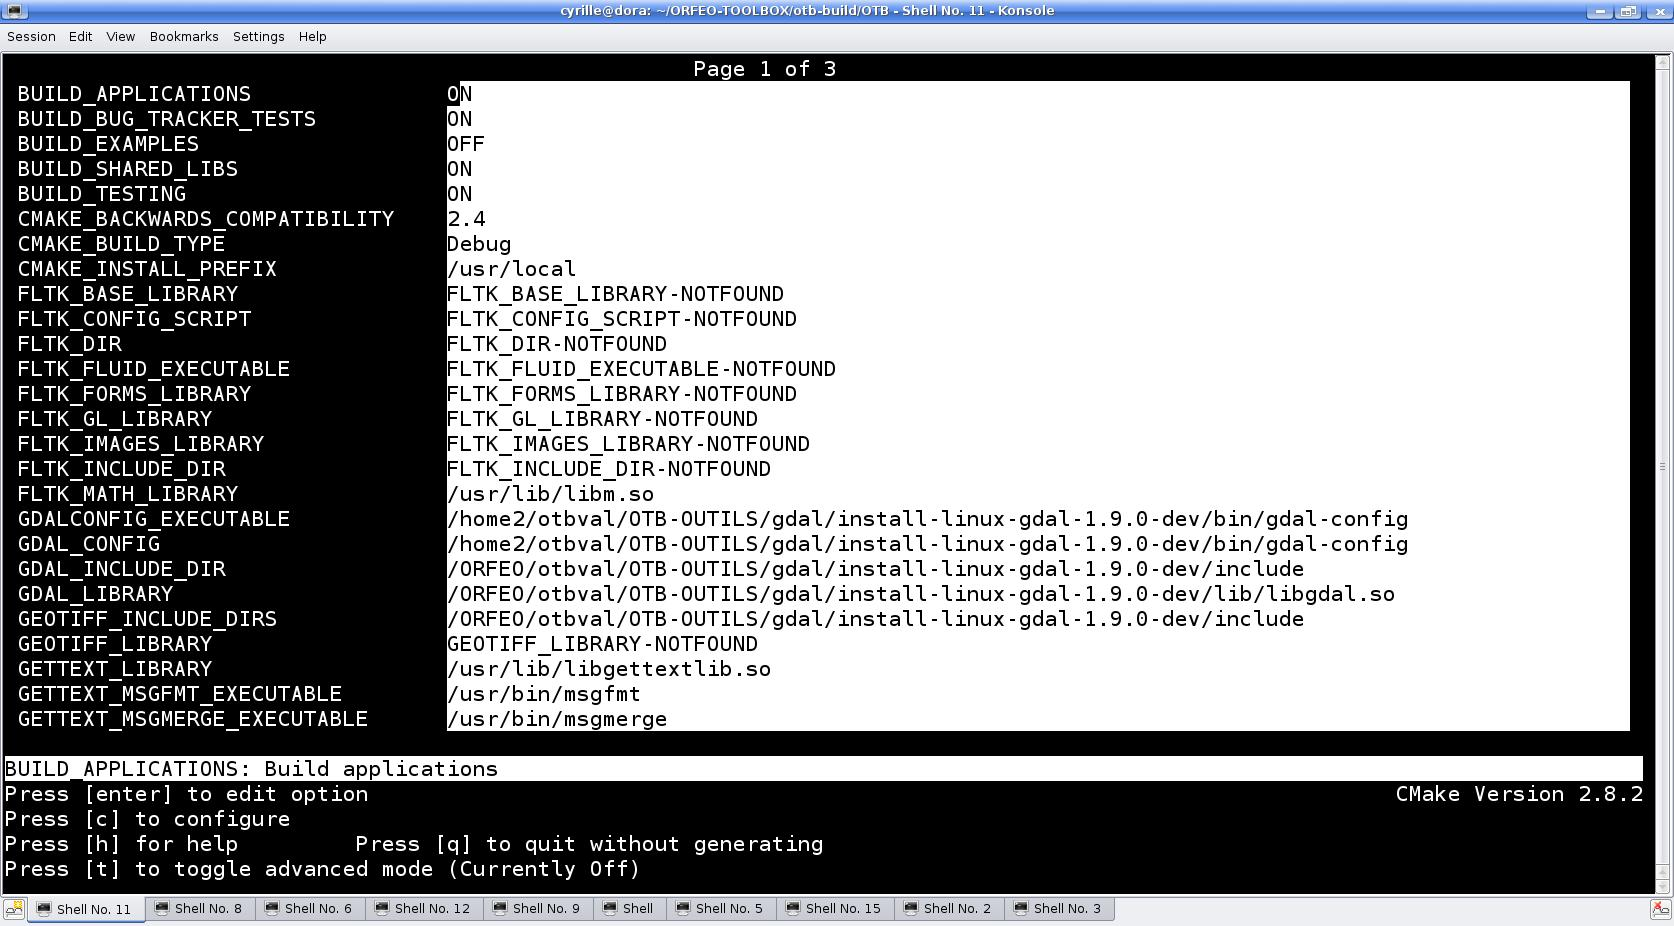
\includegraphics[width=0.8\textwidth]{ccmakeScreenShot.eps}
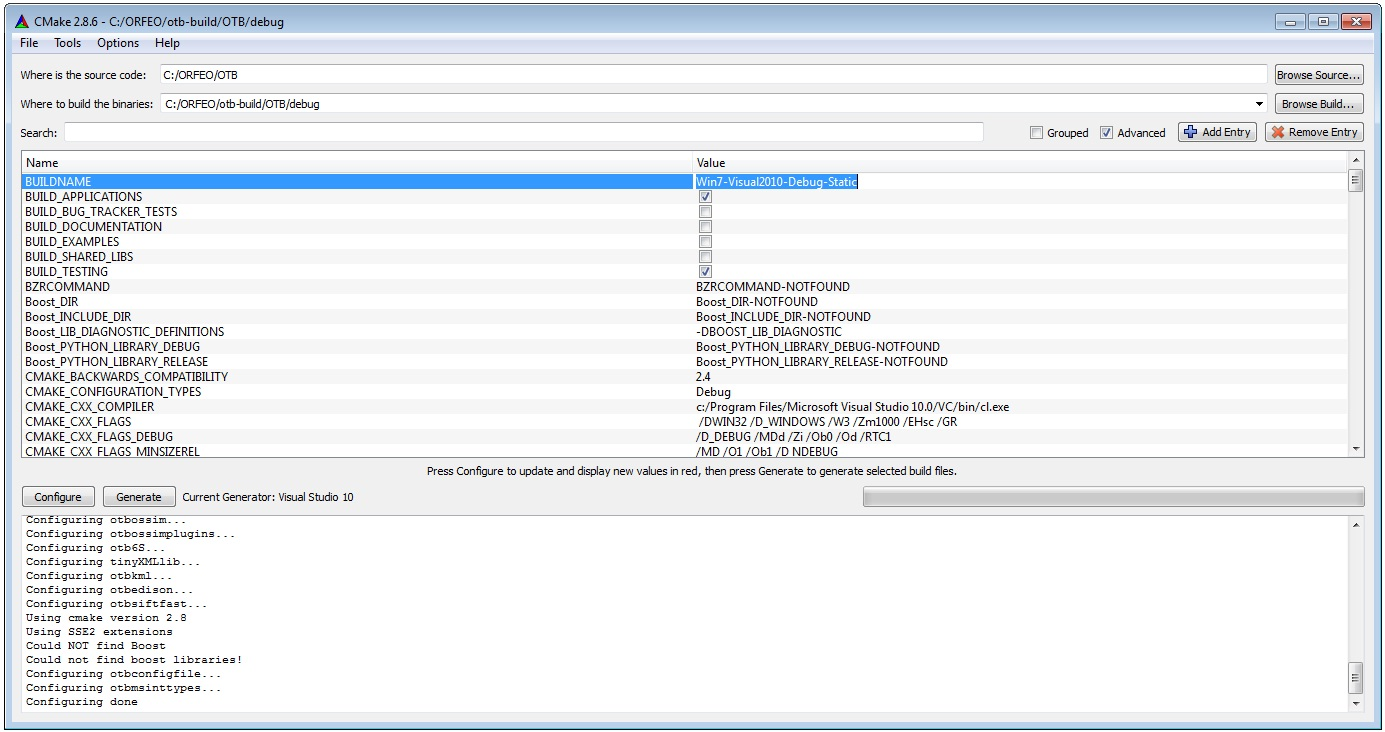
\includegraphics[width=0.8\textwidth]{CMakeSetupScreenShot.eps}
\itkcaption[Interface utilisateur de CMake]{Interface CMake. En Haut) \texttt{ccmake}, interface sous UNIX. En Bas) \texttt{CMakeSetup}, 
la version MS-Windows pour les MFC.}
\label{fig:CMakeGUI}
\end{figure}

Il est possible de choisir si l'on souhaite compiler les exemples (\code{OTB/Examples}) et les tests (\code{OTB/Testing}).
Ceci est possible en positionnant les variables \code{BUILD\_EXAMPLES=OFF} et \code{BUILD\_TESTING=OFF}.

Ces exemples peuvent \^{e}tre utilis\'{e}s pour se familiariser avec l'OTB. Les tests sont constitu\'{e}s 
d'un ensemble de petits programmes permettant de valider l'OTB.
De plus, le composant \code{OTB-Applications} montrent des applications plus \'{e}volu\'{e}es, utilisant notamment des IHM 
graphiques et de la visualisation.


\section{D\'{e}marrer avec l'OTB}
\label{sec:GettingStartedWithOTB}
 
\subsection{Hello World !}
\label{sec:HelloWorldOTB}

\index{Hello World}

Cet exemple permet de montrer comment cr\'{e}er un petit programme, qui utilise la biblioth\`{e}que OTB 
(cet exemple se trouve dans le r\'{e}pertoire \code{OTB/Examples/Installation}).
Le fichier \code{CMakeLists.txt} contient les lignes suivantes :

\small
\begin{verbatim}
PROJECT(HelloWorld)

FIND_PACKAGE(OTB)
IF(OTB_FOUND)
  INCLUDE(${OTB_USE_FILE})
ELSE(OTB_FOUND)
  MESSAGE(FATAL_ERROR
          "OTB non trouvee. Positionner la variable OTB_DIR.")
ENDIF(OTB_FOUND)

ADD_EXECUTABLE(HelloWorld HelloWorld.cxx )

TARGET_LINK_LIBRARIES(HelloWorld OTBCommon)
\end{verbatim}
\normalsize

La premi\`{e}re ligne d\'{e}finie le nom du projet pour l'environnement Visual Studio (n'a aucun effet sous UNIX).
 La seconde ligne pr\'{e}cise que la biblioth\`{e}que OTB est n\'{e}cessaire pour compiler ce programme. 
Si elle n'est pas trouv\'{e}e, un message d'erreur est \'{e}mis.
La ligne \code{ADD\_EXECUTABLE} permet de d\'{e}finir le programme que l'on cr\'{e}\'{e}e 
(le premier argument est le nom de l'ex\'{e}cutable, les suivants le(s) fichier(s) source(s) associ\'{e}(s) \`{a} cet ex\'{e}cutable)
La ligne \code{TARGET\_LINK\_LIBRARIES} pr\'{e}cise quelles biblioth\`{e}ques sont n\'{e}cessaires pour g\'{e}n\'{e}rer cet ex\'{e}cutable.

\input HelloWorld.tex

Vous avez maintenant install\'{e} et compil\'{e} avec succ\`{e}s la biblioth\`{e}que OTB, et vous avez cr\'{e}\'{e} un programme simple se \emph{linkant} avec cette biblioth\`{e}que.
Si vous avez des difficult\'{e}s, vous pouvez prendre contact avec les auteurs de ce document.

